\documentclass[reprint,twocolumn,notitlepage,superscriptaddress,floatfix]{revtex4-2}
\usepackage[T1]{fontenc}
\usepackage{amsmath,amssymb,amsthm,bm}
\usepackage{booktabs}
\usepackage{graphicx}
\usepackage{microtype}
\usepackage{url}
\usepackage[hidelinks]{hyperref}
\setlength{\emergencystretch}{3em}

\newtheorem{theorem}{Theorem}
\newtheorem{proposition}[theorem]{Proposition}
\newcommand{\R}{\mathbb R}
\newcommand{\I}{I}
\newcommand{\J}{J}
\newcommand{\M}{M}
\newcommand{\norm}[1]{\left\lVert #1\right\rVert}
\newcommand{\tr}{\operatorname{tr}}
\newcommand{\rank}{\operatorname{rank}}

\begin{document}

\title{Complement-Robust Sensitivity Subspaces for Repeated Quantum Objectives}
\author{Molena Huynh}
\email{molena.huynh@jmp.com}
\affiliation{North Carolina State University}
\date{August 1, 2026}

\begin{abstract}
A sensitivity subspace trained on repeated objectives can fail when a new
objective contains components outside the development task span.  We introduce
a complement-robust second moment that places a development-only innovation
radius on the unobserved orthogonal complement.  Its minimax discarded-gradient
loss has an exact spectral solution.  We also prove that
$\rho=\rank(\widehat M)$ transpose-Jacobian products are necessary and
sufficient for exact task-only rank-one recovery in a deterministic black-box
model, while exact robust completion uses all $m$ observable directions.  The
evaluation uses depth-one multi-angle MaxCut circuits on ten-vertex
neighborhoods drawn from eight checksum-authenticated Stanford Gset graphs.
The held-out objective factors have mean development-span distances 0.240 and
0.915 in two protocols.  At rank four, complement robustness lowers mean
held-out discarded-gradient energy from 0.0590 to 0.0381 for full objectives
and from 0.8989 to 0.4396 for localized contrasts.  The corresponding
unweighted values are 0.4858 and 0.6257.  Exact robust action is slower than
explicit dense differentiation on every tested instance.  The result is an
accuracy--cost trade-off for out-of-span transfer, with no runtime advantage
at the reported scale.
\end{abstract}

\keywords{active subspaces, QAOA, distributional robustness, Jacobian products, MaxCut}
\maketitle

\section{Sensitivity loss}

Let $F:\R^d\rightarrow\R^m$ be an observable map at an anchor parameter
$\theta_0$, with Jacobian $\J=DF(\theta_0)$.  A task vector $w\in\R^m$
defines $C_w(\theta)=w^TF(\theta)$ and gradient $\J^Tw$.  For a task second
moment $\M=\mathbb E[ww^T]$ and a rank-$r$ orthogonal projector $P$, define
\begin{equation}
 \mathcal L_{\M}(P)=
 \mathbb E\norm{(\I-P)\J^Tw}_2^2
 =\tr\!\left[\M\J(\I-P)\J^T\right].                 \label{eq:loss}
\end{equation}
If $\M=LL^T$, the loss is
$\norm{(\I-P)\J^TL}_F^2$.  Its minimizer is the dominant rank-$r$
eigenspace of $\J^T\M\J$, with minimum equal to the discarded eigenvalue sum.
This is the standard active-subspace construction
\cite{constantine2014active,constantine2015active,ipsen2009numerical}.

Development tasks $w_1,\ldots,w_s$ define
\begin{equation}
 \widehat\M=\frac1s\sum_{i=1}^s w_iw_i^T,\qquad
 \mathcal S=\operatorname{range}(\widehat\M),\qquad
 \Pi=\Pi_{\mathcal S}.                               \label{eq:source}
\end{equation}
For a held-out factor $L_t$, the dimensionless audit quantity
\begin{equation}
 \eta_{\mathcal S}(L_t)=
 \frac{\norm{(\I-\Pi)L_t}_F}{\norm{L_t}_F}           \label{eq:span}
\end{equation}
separates new task directions from new linear combinations of known
directions.

\begin{proposition}[span-transfer bound]
\label{prop:span}
For every orthogonal projector $P$,
\begin{equation}
 \sqrt{\mathcal L_{L_tL_t^T}(P)}
 \le\norm{(\I-P)\J^T\Pi L_t}_F
   +\norm{\J}_2\norm{(\I-\Pi)L_t}_F.                 \label{eq:spanbound}
\end{equation}
\end{proposition}

\begin{proof}
Insert $L_t=\Pi L_t+(\I-\Pi)L_t$ into the Frobenius representation of
Eq.~\eqref{eq:loss}, apply the triangle inequality, and use
$\norm{\I-P}_2=1$ on the second term.
\end{proof}

\section{Complement-robust construction}

An empirical task moment has no mass on $\mathcal S^\perp$.  We represent
unseen nonnegative mass by the one-sided set
\begin{equation}
 \mathcal U_\delta=
 \{\widehat\M+\Delta:\ 0\preceq\Delta
             \preceq\delta(\I-\Pi)\}.                \label{eq:set}
\end{equation}
The radius is fixed without held-out outcomes:
\begin{equation}
 \widehat\delta=\frac1s\sum_{i=1}^s
 \norm{(\I-\Pi_{-i})w_i}_2^2,                        \label{eq:radius}
\end{equation}
where $\Pi_{-i}$ projects onto all development tasks except $w_i$.

\begin{theorem}[exact complement-robust loss]
\label{thm:robust}
For every orthogonal projector $P$,
\begin{align}
 \sup_{N\in\mathcal U_\delta}\mathcal L_N(P)
 &=\mathcal L_{\widehat\M}(P)
 +\delta\norm{(\I-\Pi)\J(\I-P)}_F^2                 \notag\\
 &=\mathcal L_{\widehat\M+\delta(\I-\Pi)}(P).        \label{eq:identity}
\end{align}
The minimizing rank-$r$ projector is a dominant eigenspace of
\begin{equation}
 H_\delta=\J^T[\widehat\M+\delta(\I-\Pi)]\J.          \label{eq:hessian}
\end{equation}
If $s^{-1/2}[w_1,\ldots,w_s]=U\Sigma V^T$ is compact and
$U_\perp$ spans $\mathcal S^\perp$, then
\begin{equation}
 B_\delta=\J^T[U\Sigma,\sqrt{\delta}\,U_\perp],
 \qquad B_\delta B_\delta^T=H_\delta.                \label{eq:factor}
\end{equation}
\end{theorem}

\begin{proof}
Let $R=\J(\I-P)$ and $K=RR^T\succeq0$.  Feasibility gives
\begin{equation}
 \tr(\Delta K)\le\delta\tr[(\I-\Pi)K],
\end{equation}
because $\delta(\I-\Pi)-\Delta\succeq0$.  Equality is attained by
$\Delta=\delta(\I-\Pi)$, proving Eq.~\eqref{eq:identity}.  The usual
trace-maximization argument gives Eq.~\eqref{eq:hessian}.  Finally,
$U\Sigma^2U^T=\widehat\M$ and
$U_\perp U_\perp^T=\I-\Pi$, which proves Eq.~\eqref{eq:factor}.
\end{proof}

For normalized development tasks, $0\le\widehat\delta\le1$; it is invariant
under task permutation and orthogonal observable-coordinate changes.  It is a
source-coverage diagnostic, not a distribution-free probability guarantee.

\section{Derivative-query bound}

Let $\rho=\rank(\widehat\M)$ and define the task-only factor
\begin{equation}
 B=\J^TU\Sigma\in\R^{d\times\rho}.                   \label{eq:taskfactor}
\end{equation}
Each column is one transpose-Jacobian product.

\begin{theorem}[exact deterministic query complexity]
\label{thm:query}
In a black-box model returning $\J^Tv$ for a queried $v\in\R^m$, exactly
$\rho$ queries are necessary and sufficient to recover the unique leading
task-only sensitivity direction for every $\J$ when $d\ge2$.  Exact
complement robustness with $\delta>0$ uses $m$ queries through
Eq.~\eqref{eq:factor}.  Task-only construction costs
\begin{equation}
 O\!\left(ms\min\{m,s\}+\rho T_{\rm VJP}+d\rho^2\right)
                                                               \label{eq:cost}
\end{equation}
and stores $O(ms+d\rho)$ numbers.
\end{theorem}

\begin{proof}
The identity
\begin{equation}
 \J^T\widehat\M\J=\J^TU\Sigma^2U^T\J=BB^T
\end{equation}
proves sufficiency.  Suppose an adaptive deterministic procedure makes
$k<\rho$ queries and receives zero each time.  A nonzero
$z\in\mathcal S$ exists orthogonal to every query.  For orthogonal unit
vectors $a,b\in\R^d$, the two maps
$\J_a^T=az^T$ and $\J_b^T=bz^T$ produce the same transcript, while their
unique leading sensitivity spaces are respectively $\operatorname{span}(a)$
and $\operatorname{span}(b)$.  No common output is correct, so $k\ge\rho$.
The robust factor has $\rho+(m-\rho)=m$ columns.  A compact task SVD, the
$\rho$ products, and a thin SVD of the $d\times\rho$ factor give
Eq.~\eqref{eq:cost} and its storage count.
\end{proof}

\section{Authenticated experiment}

The study uses G1, G6, G11, G14, G18, G22, G32, and G43 from Stanford Gset
\cite{ye2003gset}.  Every graph file is accepted only after its SHA-256 digest
matches the registered value.  A deterministic breadth-first rule selects one
ten-vertex induced neighborhood per source.  The observable vector contains
edge-cut expectations of a depth-one multi-angle QAOA circuit
\cite{farhi2014qaoa,hadfield2019alternating,herrman2022multiangle}.
Complex-double state-vector differentiation supplies matched action and dense
Jacobians.

Two five-task held-out protocols are fixed before scoring.  Full objectives
mix every edge observable and have mean span residual 0.240.  Localized
contrasts emphasize source-absent observable directions and have mean residual
0.915.  A rejected vector split, retained only as a leakage control, has
maximum residual $6.83\times10^{-16}$.  The rank-four comparison includes
task-only, unweighted observable, coordinate-energy, and complement-robust
subspaces.

\begin{table}[t]
\caption{\label{tab:loss}Mean normalized discarded-gradient energy at rank
four.  Training and held-out columns are reported separately; lower is better.}
\centering\scriptsize
\begin{tabular}{llrr}\toprule
Protocol & Method & train & held-out \\
\midrule
Full objective & Complement-robust & 0.0149 & 0.0381 \\
Full objective & Task-only active subspace & 0.0014 & 0.0590 \\
Full objective & Unweighted observable SVD & 0.4658 & 0.4858 \\
Full objective & Coordinate energy & 0.4363 & 0.4788 \\
\midrule
Localized contrast & Complement-robust & 0.9789 & 0.4396 \\
Localized contrast & Task-only active subspace & 0.0686 & 0.8989 \\
Localized contrast & Unweighted observable SVD & 0.5166 & 0.6257 \\
Localized contrast & Coordinate energy & 0.4864 & 0.9306 \\
\bottomrule\end{tabular}

\end{table}

Table~\ref{tab:loss} exhibits the robustness trade-off.  On full objectives,
complement completion reduces held-out energy by 35.4\% relative to task-only.
On localized contrasts, the reduction is 51.1\%.  Its contrast training loss
is much larger, as expected when the model reserves capacity for
$\mathcal S^\perp$.  The method improves the mean on all eight contrast
targets relative to task-only; it does not beat every baseline on every graph.
Figure~\ref{fig:transfer} displays the corresponding rank path and paired
target losses.

\begin{figure*}[t]
\centering
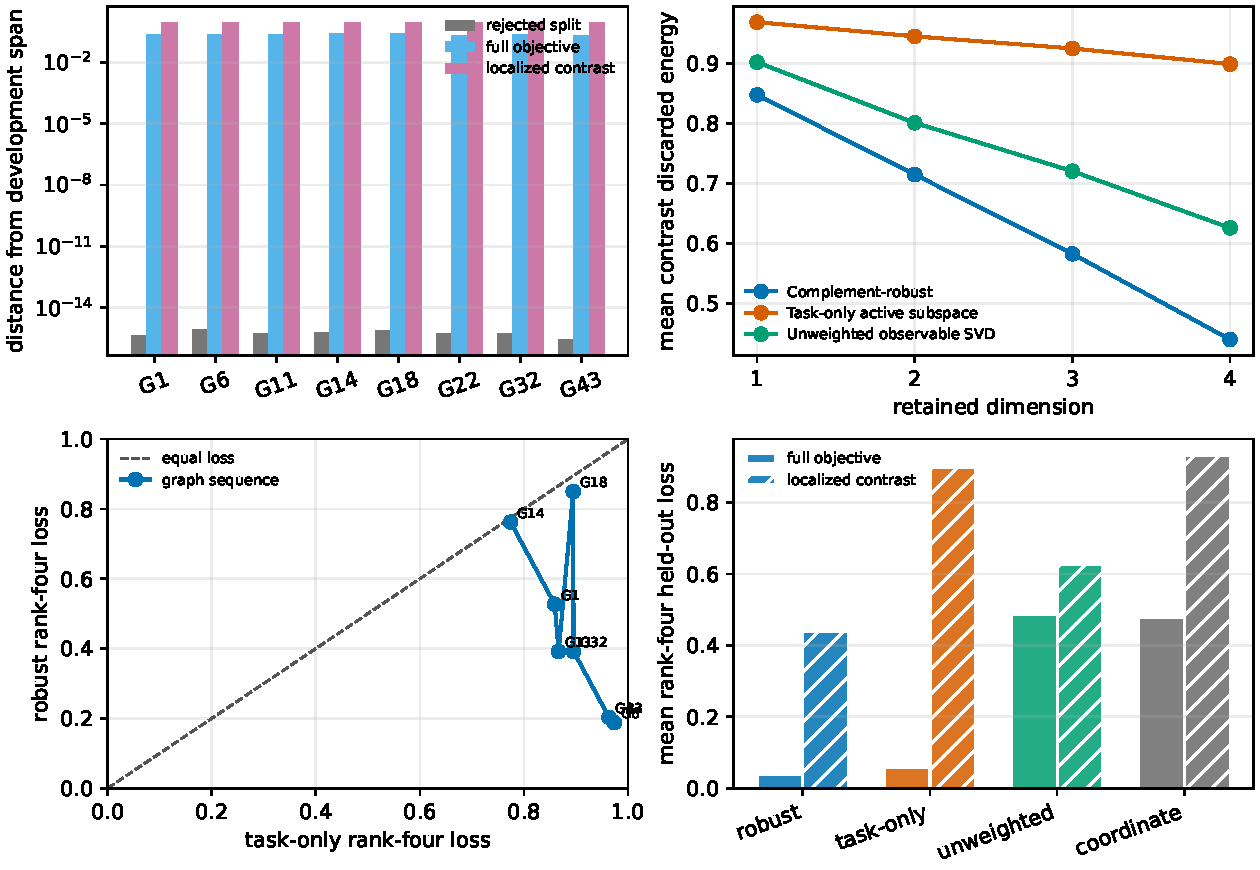
\includegraphics[width=0.95\textwidth]{code/manuscript_assets/figures/robust_transfer_audit.pdf}
\caption{\label{fig:transfer}Out-of-span transfer audit.  Top left: development
span distance for the leakage control and two registered protocols.  Top
right: contrast loss across retained ranks.  Bottom left: paired rank-four
task-only and robust losses; points below the diagonal favor completion.
Bottom right: aggregate held-out loss under both protocols.}
\end{figure*}

The action and dense constructions agree in objective value to at least
$1.1\times10^{-15}$ on the rank-four checks.  This agreement validates the
factorizations in Theorems~\ref{thm:robust} and \ref{thm:query}; it does not
establish speed.  The task-only method uses five products on every graph,
whereas robust completion uses 9--21.  On the locked CPU run, robust action is
1.33--1.40 times slower than matched dense robust construction;
Fig.~\ref{fig:cost} and Table~\ref{tab:resource} separate derivative counts,
wall time, dimensions, and numerical agreement.

\begin{figure*}[t]
\centering
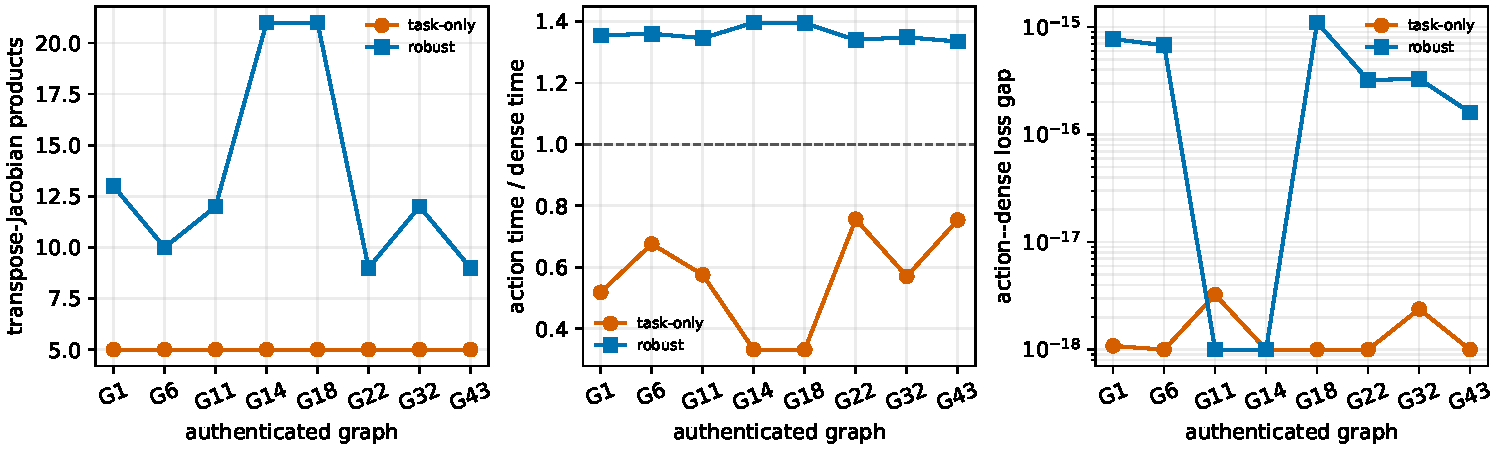
\includegraphics[width=0.96\textwidth]{code/manuscript_assets/figures/oracle_cost_audit.pdf}
\caption{\label{fig:cost}Derivative and implementation audit.  Left:
transpose-Jacobian counts predicted by Theorem~\ref{thm:query}.  Center:
action-to-dense runtime ratio, with unity marking equal time.  Right:
action--dense rank-four objective gaps for the factorizations in
Theorems~\ref{thm:query} and \ref{thm:robust}.}
\end{figure*}

\begin{table}[t]
\caption{\label{tab:resource}Dimensions and exact transpose-Jacobian counts.
Here $m$ is the number of local edge observables, $d$ the parameter dimension,
and $\rho$ the development-moment rank.}
\centering\scriptsize
\begin{tabular}{lrrrrr}\toprule
Graph & $m$ & $d$ & $\rho$ & task VJP & robust VJP \\
\midrule
G1 & 13 & 23 & 5 & 5 & 13 \\
G6 & 10 & 20 & 5 & 5 & 10 \\
G11 & 12 & 22 & 5 & 5 & 12 \\
G14 & 21 & 31 & 5 & 5 & 21 \\
G18 & 21 & 31 & 5 & 5 & 21 \\
G22 & 9 & 19 & 5 & 5 & 9 \\
G32 & 12 & 22 & 5 & 5 & 12 \\
G43 & 9 & 19 & 5 & 5 & 9 \\
\bottomrule\end{tabular}

\end{table}

\section{Reproducibility and scope}

The repository records graph addresses and hashes, selected vertex identifiers,
task vectors, span residuals, innovation radii, all rank frontiers, adjointness
checks, action--dense gaps, derivative counts, and repeated timings.  The
offline replay recomputes all eight circuits, verifies every registered
finding against the locked result, and regenerates the tables and figures.

The evidence concerns ten-qubit, depth-one, noiseless state-vector objectives.
It does not imply hardware performance, global MaxCut quality, or a runtime
benefit.  Its supported conclusion is narrower: complement-supported moment
completion improves out-of-span gradient preservation on the registered graph
panel, at the disclosed derivative and wall-clock cost.

\bibliographystyle{apsrev4-2}
\bibliography{code/manuscript_assets/references}

\end{document}
